\documentclass[12pt,addpoints]{exam}
\usepackage{graphicx}
\usepackage{amsmath}
\usepackage{amssymb}
\usepackage{hyperref}

\linespread{1.25}
\extrawidth{.75in}
\setlength\linefillheight{.5in}

\pagestyle{headandfoot}

\runningheadrule
\firstpageheader
    {CSC 212 / URI}
    {Final Exam}
    {Dec 19, 2020}
\runningheader
    {CSC 212 / URI}
    {Final Exam, Page \thepage\ of \numpages}
    {Dec 19, 2020}
\firstpagefooter
    {}
    {}
    {}
\runningfooter
    {}
    {}
    {}

\begin{document}

~{\large
    \vspace{.5in}

    This exam has \numquestions\ questions, for a total of \numpoints\ points.  You have 2.5 hours to complete the exam.  Please read carefully the guidelines below:

    \begin{itemize}
        \item[-] Your submission to Gradescope must include the following files:
        \begin{enumerate}
            \item A text file named \verb|XXXX.txt|, where \verb|XXXX| are the last four digits of your {\bf student ID}.  \underline{This file is the most important} as it will be used for {\bf grading} your work.  This file must contain your final answers to all questions, one per line.  If you don't have an answer, you can leave the line empty.  A template is provided at: \url{https://homepage.cs.uri.edu/~malvarez/stationary/exam/ans.txt}.
            \item A PDF file named \verb|XXXX.pdf|, where \verb|XXXX| are the last four digits of your {\bf student ID}.  This file will contain your work.  You can write your solutions on your own paper(s) and then scan or photograph them into a single PDF.  Do not worry about alignment or format, as long as your work is readable. In this file, your work on each question can be in any order.
        \end{enumerate}
        \item[-] If the question is multiple choice, the answer {\bf must be} the corresponding letter (A, B, C, ...).  If the question is open, the answer will be a single number, or as otherwise specified in the question.
        \item[-] You may use any of our lecture notes, books, or additional written/online references.  However, when solving the questions, your solution must follow the algorithms and formulas introduced in our lectures.
    \end{itemize}
    
    By submitting my solutions to this exam I acknowledge that I have read and understood the guidelines above, that all answers are my own, and that I have neither gained unfairly from others nor have I assisted others in obtaining an unfair advantage.
}

\pagebreak

\begin{questions}

\question[5] 
Consider an empty hash table of length $11$, in which keys $17,22,1,32,23,41,9,28$ are inserted with $h(x)=(x+5) \mod 11$ and separate chaining.  What is the total number of {\it collisions}?
\answerline

\question[5] 
A post-order traversal of a {\it max-heap} with $7$ elements is $1,2,\dots,6,7$.  What is the sum of all nodes of height $h=1$?
\answerline

\question[5] Considering the BST below:
\begin{figure}[h!]
  \centering
  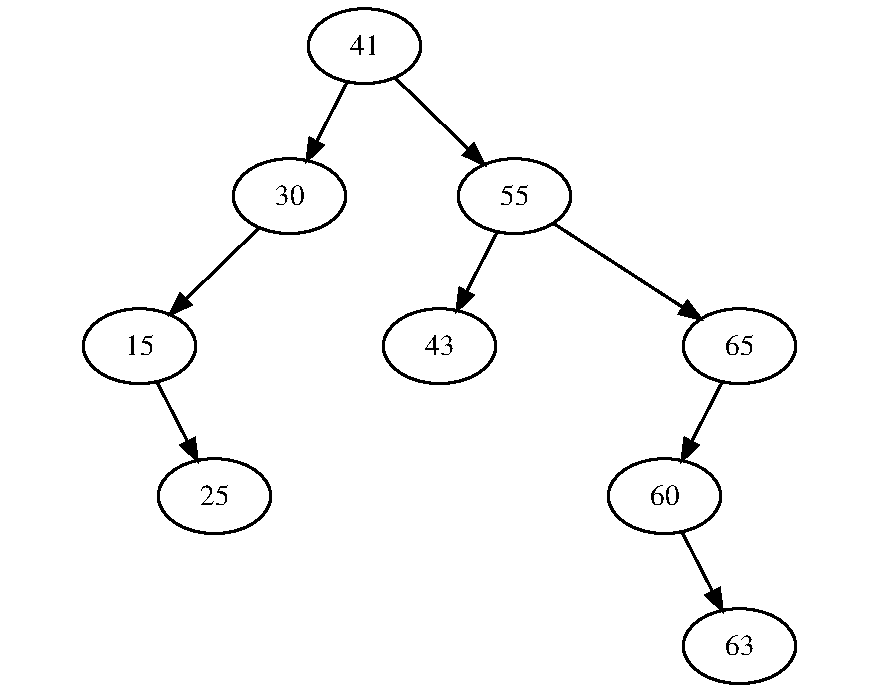
\includegraphics[height=2.5in]{imgs/bst.pdf}
\end{figure}

What is the output of a preorder traversal that, for each visit, prints the {\it height} of the node?
\begin{choices}	
	\choice None of the others	
	\choice 4, 3, 2, 1, 0, 1, 0, 3, 2, 1, 0	
	\choice 4, 3, 2, 2, 2, 1, 4, 3, 2, 1, 0	
	\choice 4, 3, 2, 3, 2, 1, 4, 2, 2, 1, 0	
	\choice 4, 3, 2, 1, 0, 1, 1, 3, 2, 1, 0
\end{choices}
\answerline

\question[5] 
Indicate the sum of the values corresponding to all statements that are \verb|True|.  Mark $0$ if none are \verb|True|:
\begin{itemize}
	\item[$(1)$] Traversing a BST using {\it pre-order} results in a sorted list of keys
	\item[$(2)$] The worst-case performance of finding the largest element of a BST is $\Theta(1)$
	\item[$(4)$] A binary heap is a complete BST
	\item[$(8)$] $2^h$ is the minimum number of nodes in a binary heap of height $h$\end{itemize}
\answerline

\end{questions}

\end{document}